%%%%%%%%%%%%%%%%%%%%%%%%%%%%%%%%%%%%%%%%%%%%%%%%%%%%%%%%%%%%%%%%%%%%%%
% LaTeX Template: Designer's CV
%
% Source: http://www.howtotex.com
% 
% Feel free to distribute this example, but please keep the referral
% to HowToTeX.com
% 
% Date: March 2012 
%
% Modified by Lim Lian Tze to support multiple pages using fix provided at
% http://www.howtotex.com/templates/creating-a-designers-cv-in-latex/
% Date: November 2014
%%%%%%%%%%%%%%%%%%%%%%%%%%%%%%%%%%%%%%%%%%%%%%%%%%%%%%%%%%%%%%%%%%%%%%
% How to use writeLaTeX: 
%
% You edit the source code here on the left, and the preview on the
% right shows you the result within a few seconds.
%
% Bookmark this page and share the URL with your co-authors. They can
% edit at the same time!
%
% You can upload figures, bibliographies, custom classes and
% styles using the files menu.
%
% If you're new to LaTeX, the wikibook is a great place to start:
% http://en.wikibooks.org/wiki/LaTeX
%
%%%%%%%%%%%%%%%%%%%%%%%%%%%%%%%%%%%%%%%%%%%%%%%%%%%%%%%%%%%%%%%%%%%%%%

%%%%%%%%%%%%%%%%%%%%%%%%%%%%%%%%%%%%%
% Document properties and packages
%%%%%%%%%%%%%%%%%%%%%%%%%%%%%%%%%%%%%
\documentclass[a4paper,12pt,final]{memoir}
\usepackage[spanish]{babel}
\usepackage[utf8]{inputenc}

% misc
\renewcommand{\familydefault}{bch}	% font
\pagestyle{empty}					% no pagenumbering
\setlength{\parindent}{0pt}			% no paragraph indentation


% required packages (add your own)
\usepackage{flowfram}										% column layout
\usepackage[top=1cm,left=1cm,right=1cm,bottom=1cm]{geometry}% margins
\usepackage{graphicx}										% figures
\usepackage{url}											% URLs
\usepackage[usenames,dvipsnames]{xcolor}					% color
\usepackage{multicol}										% columns env.
	\setlength{\multicolsep}{0pt}
\usepackage{paralist}										% compact lists
\usepackage{tikz}

%%%%%%%%%%%%%%%%%%%%%%%%%%%%%%%%%%%%%
% Create column layout
%%%%%%%%%%%%%%%%%%%%%%%%%%%%%%%%%%%%%
% define length commands
\setlength{\vcolumnsep}{\baselineskip}
\setlength{\columnsep}{\vcolumnsep}

% left frame
\newflowframe{0.2\textwidth}{\textheight}{0pt}{0pt}[left]
	\newlength{\LeftMainSep}
	\setlength{\LeftMainSep}{0.2\textwidth}
	\addtolength{\LeftMainSep}{1\columnsep}
 
% small static frame for the vertical line
\newstaticframe{1.5pt}{\textheight}{\LeftMainSep}{0pt}
 
% content of the static frame
\begin{staticcontents}{1}
\hfill
\tikz{%
	\draw[loosely dotted,color=RoyalBlue,line width=1.5pt,yshift=0]
	(0,0) -- (0,\textheight);}%
\hfill\mbox{}
\end{staticcontents}
 
% right frame
\addtolength{\LeftMainSep}{1.5pt}
\addtolength{\LeftMainSep}{1\columnsep}
\newflowframe{0.7\textwidth}{\textheight}{\LeftMainSep}{0pt}[main01]


%%%%%%%%%%%%%%%%%%%%%%%%%%%%%%%%%%%%%
% define macros (for convience)
%%%%%%%%%%%%%%%%%%%%%%%%%%%%%%%%%%%%%
\newcommand{\Sep}{\vspace{1.5em}}
\newcommand{\SmallSep}{\vspace{0.5em}}

\newenvironment{AboutMe}
	{\ignorespaces\textbf{\color{RoyalBlue} Descripción.}}
	{\Sep\ignorespacesafterend}
	
\newcommand{\CVSection}[1]
	{\Large\textbf{#1}\par
	\SmallSep\normalsize\normalfont}

\newcommand{\CVItem}[1]
	{\textbf{\color{RoyalBlue} #1}}


%%%%%%%%%%%%%%%%%%%%%%%%%%%%%%%%%%%%%
% Begin document
%%%%%%%%%%%%%%%%%%%%%%%%%%%%%%%%%%%%%
\begin{document}

% Left frame
%%%%%%%%%%%%%%%%%%%%
%
% Upload your own photo using the files menu
\begin{figure}
	\hfill
	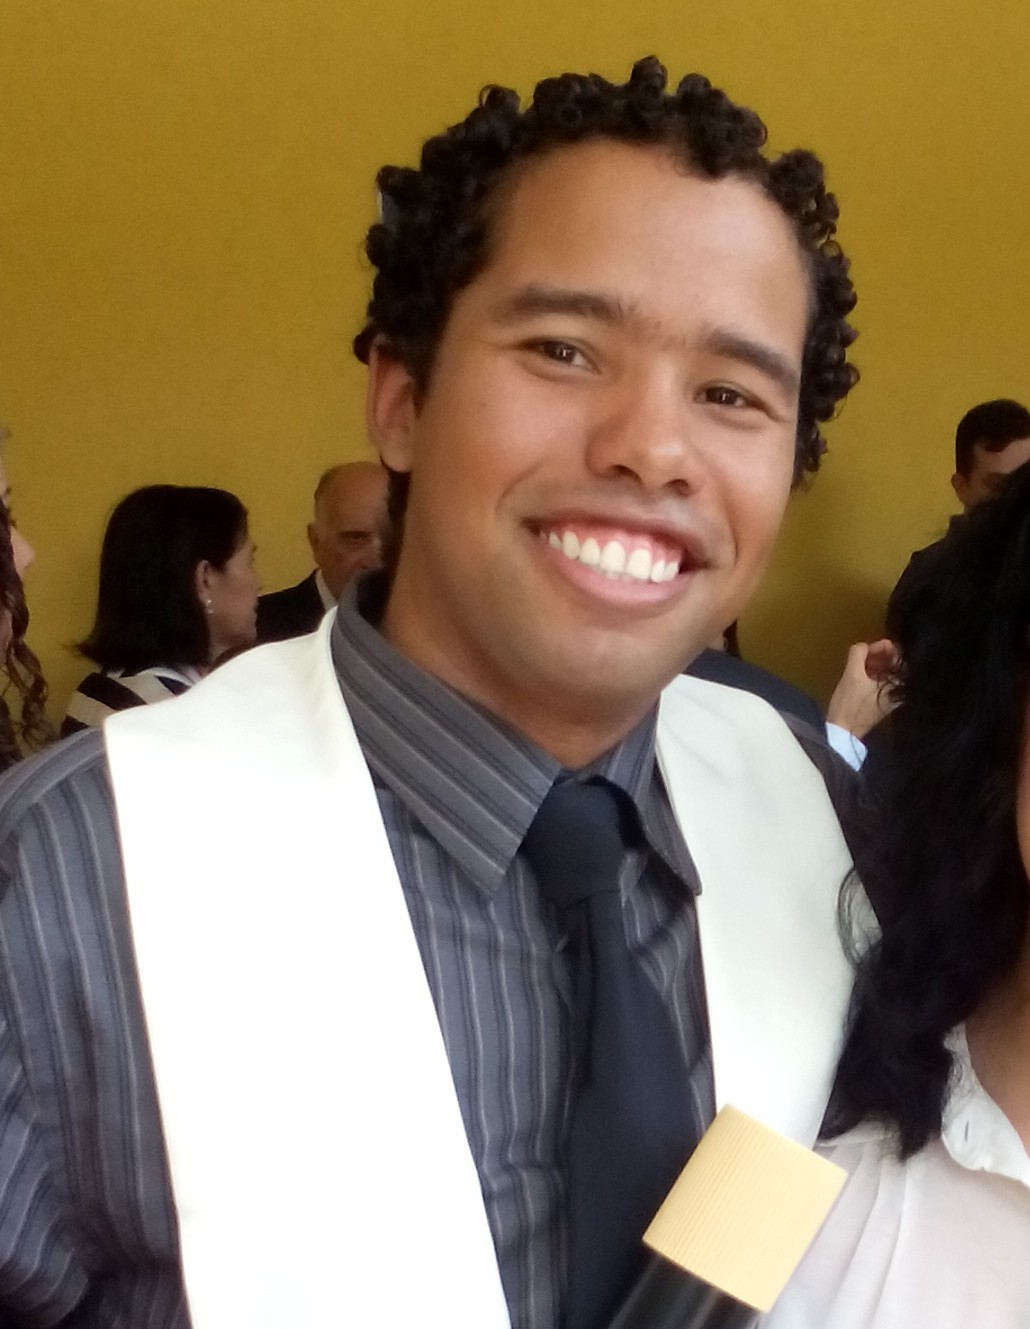
\includegraphics[width=0.8\columnwidth]{foto.jpg}
	\vspace{-7cm}
\end{figure}

\begin{flushright}\small
	Esteban M. Díaz T. \\
	\tiny{\url{esteban.diazt23@gmail.com}}\\
	9 9515-6801 
\end{flushright}\normalsize
\framebreak


% Right frame
%%%%%%%%%%%%%%%%%%%%
\Huge\bfseries {\color{RoyalBlue} Esteban M. Díaz T.} \\
\Large\bfseries  Computista / Programador \\

\normalsize\normalfont

% About me
\begin{AboutMe}
Licenciado en ciencias de la computación (programador) con 5 años de experiencia
en la solución de problemas diversos mediante el uso de tecnología y herramientas
informáticas, aplicando mis conocimientos para dar un mayor impulso a su empresa.
Ávido por adquirir nuevos conocimientos y aprender nuevas tecnologías para
aplicarlas en conjunto.
\end{AboutMe}

\CVSection{Información Personal}
\setlength{\columnsep}{-3.5cm}      % separacion de las columnas en multicols
\begin{multicols}{2}
RUT: \\
Nacionalidad: \\
Fecha de Nacimiento: \\
Edad: \\
Estado Civil: \\
Dirección: \\
\newline
Teléfono: \\
Correo Electrónico: \\
\vfill
\columnbreak
26.598.186-0\\
Venezolano.\\
23 de octubre de 1992.\\
27 Años.\\
Soltero.\\
Santiago, Comuna San Miguel, Calle Alcalde Pedro Alarcón 844, Departamento 603.\\
9 9515-6801 \\
esteban.diazt23@gmail.com
\end{multicols}

\Sep

% Experiencia laboral
\CVSection{Experiencia Laboral}
\CVItem{2019 - Presente. Acruxlab S.P.A}\\
Desarrollo sobre el sistema odoo versión 8 y 11 que incluye:
\begin{compactitem}[\color{RoyalBlue}$\circ$]
	\item Adaptación a las necesidades específicas del cliente.
	\item Desarrollo de nuevas herramientas.
	\item Integración con sistemas externos.
	\item Adaptaciones y desarrollos sobre la sección POS (punto de venta).
\end{compactitem}

\SmallSep

\CVItem{2016 - 2018. Analista Programador. Ford Motor de Venezuela}\\
Migracion de las plataformas informáticas de la empresa basada en herramientas
Oracle a tecnología web, utilizando el siguiente stack:
\begin{compactitem}[\color{RoyalBlue}$\circ$]
	\item Lenguaje de programación Java bajo el framework JSF.
	\item Primefaces como framework para front-end.
	\item Persistencia de datos con JPA/Eclipselink.
	\item Almacenando la informacion en base de datos Oracle.
\end{compactitem}
Contrato bajo la empresa Sluxnet c.a.

\SmallSep

\CVItem{2015 - 2016. Analista Programador - Corporacion Inlaca}\\
Analista programar de soluciones de software para plataforma web utilizando los
Siguientes lenguajes y herramientas:
\begin{compactitem}[\color{RoyalBlue}$\circ$]
	\item Classic ASP
	\item PL/SQL
	\item Javascript, hmlt y css
	\item Base de datos Oracle
\end{compactitem}
Contrato bajo la empresa Sluxnet c.a.

\newpage
.
\normalsize
\framebreak

% Education
\CVSection{Educación}
\CVItem{2009 - Presente, Universitaria - Universidad de Carabobo}\\
Cursando 10mo semestre en Ciencias de la Computación en la Facultad Experimental
de Ciencias y Tecnología (FACyT).
\SmallSep

\CVItem{2004 - 2009, Secundaria - U. E. Enrique Tejera}\\
Titulo obtenido - Bachiller en Ciencias.
\SmallSep

\CVItem{1999 - 2004, Primaria - E. B. Dr. Carlos Arvelo}\\
Titulo obtenido - Certificado de primaria.

\Sep

\CVSection{Cursos Realizados}
\CVItem{2008 - Guacara, FUNDAUC}\\
Idiomas Modernos, Ingles Básico.
\Sep

% You'll need these 3 lines at the end of each page!
%\clearpage
%\framebreak
%\framebreak

% Skills
\CVSection{Habilidades}
\begin{multicols}{3}
\begin{compactitem}[\color{RoyalBlue}$\circ$]
	\item Responsable.
	\item Proactivo. 
	\item Puntual.
	\item Honesto.
	\item Trabajo en equipo.
	\item \dots
\end{compactitem}
\end{multicols}
\SmallSep

\CVItem{Lenguajes de Programación utilizados}
\begin{multicols}{2}
\begin{compactitem}[\color{RoyalBlue}$\circ$]
	\item C/C++ 
	\item PHP 
	\item Java
	\item SQL (MySql y PostgreSQL) 
\end{compactitem}
\end{multicols}
\Sep 

% References
%\CVSection{References}

%%%%%%%%%%%%%%%%%%%%%%%%%%%%%%%%%%%%%
% End document
%%%%%%%%%%%%%%%%%%%%%%%%%%%%%%%%%%%%%
\end{document}